% !TeX root = ../thesis.tex
\chapter{Results}
\label{chap:results}

This chapter reports the reconciled historical evidence, the official three-checkpoint test results, the validation-only prototype-distance and normal-bag studies, and the dense temporal/system evaluation. Unless a result is explicitly identified as historical or validation-only, numerical values refer to the fixed UCF-Crime test split. All means and sample standard deviations are calculated over the three independently trained Stage-2 checkpoints with seeds 1337, 2027, and 3407. These three values describe between-checkpoint variability; the 870 checkpoint--video outputs are not treated as independent replicates. For three headline quantities, a 95\% paired video bootstrap interval is added (Section~\ref{sec:evaluation-paths}). It describes the uncertainty from the particular 290 test videos and does not include training variance. No significance test is made.

\section{Evaluation Setup}
\label{sec:results-setup}
\label{sec:results-protocol}

Results below use the fixed 290-video test split (150 normal, 140 anomalous) and the three official Stage-2 checkpoints selected as described in Section~\ref{sec:optimization}. The two test input paths of Section~\ref{sec:evaluation-paths} are reported separately and never pooled: the fixed-bag path (one immutable 16-instance bag per video, 4,640 clips per checkpoint) and the dense indexed path (all 69,090 indexed clips).

Response routing uses all 290 videos unless marked otherwise; the anomaly-conditional population restricts to the 140 ground-truth anomalous videos as an oracle-conditioned diagnostic, not an operating condition. Positive response support is imbalanced: Police is positive for 119 test videos, Medical for 77, and Fire for 53. Temporal metrics exclude the five annotation-boundary videos of Section~\ref{sec:temporal-evaluation}, leaving 135 source-bounded anomalous videos; normal-video temporal summaries use all 150 normal videos.

Binary, response, and temporal metrics below follow the definitions and decision rules fixed in Sections~\ref{sec:evaluation-paths} and~\ref{sec:temporal-evaluation}: argmax over the two binary logits, independent response thresholding at 0.5, the raw/binary-gated/anomaly-conditional routing views, Response Macro-F1/Hamming loss/exact match, the all-services and binary-gated-all-services references, and the primary (threshold 0.5) versus display (threshold 0.65, gated) temporal rules. Any two rows compared below share the same input path and population unless stated otherwise.

All binary AUROC values in this thesis are video-level: each of the 290 test videos contributes one anomaly score and one label, so the value can be read as the probability that a randomly chosen anomalous video receives a higher score than a randomly chosen normal one \cite{fawcett2006introduction}. The original UCF-Crime benchmark evaluates at frame level instead, with a ROC curve over frame scores compared against the temporal annotation \cite{sultani2018real}. Because the two measures differ in their unit of evaluation and in what counts as a positive, the values reported here cannot be set beside published frame-level results. No frame-level AUROC is computed in this thesis; the published frame-level values in Table~\ref{tab:related-comparison} orient the reader and are not compared numerically.

\section{Historical 14-Class Development Outputs}
\label{sec:results-historical}

The response formulation was preceded by a 14-class task in which Normal and the 13 UCF-Crime anomaly categories were mutually exclusive classes. Two direct test outputs of that task are retained, one on frozen and one on LoRA-adapted features (Table~\ref{tab:results-historical}). The frozen-feature output assigned 282 of the 290 test videos to Normal and reached a Macro-F1 of 0.074. The later, LoRA-adapted output assigned 175 videos to Normal and distributed the remaining 115 over all 13 anomaly categories, for a Macro-F1 of 0.196. The LoRA-adapted run used the same adapted feature store and prototype memory as the official response models (Chapter~\ref{chap:methods}). Both outputs are weak, and in both most predictions are Normal. The two runs are development history, not a controlled comparison. They differ in feature and prototype-distance inputs, training settings, and checkpoint selection, and their provenance is incomplete, so the difference between them does not estimate an effect of LoRA. Neither value is compared with the three-channel response results, since the labels, objectives, decision rules, and Macro-F1 denominators of the two tasks differ.

\begin{table}[tbp]
    \centering
    \small
    \caption[Historical 14-class test outputs.]{Retained historical 14-class outputs on the 290-video test split. Each row is a single output, evaluated on one deterministic 16-instance epoch-0 bag per video with a 14-class argmax, so no three-seed mean or uncertainty applies. The rows differ in inputs, training settings, selection, and provenance and do not form a controlled LoRA comparison.}
    \label{tab:results-historical}
    \begin{tabularx}{\textwidth}{@{}lccc>{\raggedright\arraybackslash}X@{}}
        \toprule
        \textbf{Historical output} & \textbf{Accuracy} & \textbf{Macro-recall} & \textbf{Macro-F1} & \textbf{Prediction distribution} \\
        \midrule
        Frozen features & 0.528 & 0.091 & 0.074 & 282 Normal, 7 Arson, 1 Explosion \\
        LoRA-adapted features & 0.572 & 0.221 & 0.196 & 175 Normal, 115 over all 13 anomaly categories \\
        \bottomrule
    \end{tabularx}
\end{table}

\section{Official Fixed-Bag Binary Anomaly Results}
\label{sec:results-fixed-binary}

The three checkpoints were selected by validation response Macro-F1 (Section~\ref{sec:optimization}). Predicting all three services for each of the 161 validation videos gives a validation response Macro-F1 of 0.4046. The selected checkpoints reached 0.4451, 0.4287, and 0.4328 at epochs 34, 0, and 25, that is 0.040, 0.024, and 0.028 above this reference, and the per-epoch validation values of all three runs stayed close to it.

Table~\ref{tab:results-fixed-binary} gives the binary results for the official fixed bags. Mean AUROC was $0.940 \pm 0.002$ (95\% video bootstrap interval 0.910 to 0.967), while positive-class F1 was $0.875 \pm 0.012$. Recall varied more across checkpoints than precision, with sample standard deviations of 0.032 and 0.009, respectively.

\begin{table}[tbp]
    \centering
    \small
    \caption[Official fixed-bag binary test results.]{Official binary anomaly results on all 290 test videos using the immutable 16-instance fixed bags. AUROC is threshold-free and video-level; the other metrics use binary-logit argmax, with an exact tie assigned to Normal. Seed columns give the three selected Stage-2 checkpoints; for seed 2027 this is the epoch-0 checkpoint (Section~\ref{sec:optimization}). The sample SD reflects variation between Stage-2 training seeds only. The adapter, feature store, and prototypes are shared by all three checkpoints, so the SD is not an uncertainty estimate for the whole pipeline. The bootstrap interval in the text covers test-video sampling only. No temporal cases are excluded and the response threshold is not involved.}
    \label{tab:results-fixed-binary}
    \begin{tabular}{@{}lcccc@{}}
        \toprule
        \textbf{Binary metric} & \textbf{Seed 1337} & \textbf{Seed 2027} & \textbf{Seed 3407} & \textbf{Mean $\pm$ sample SD} \\
        \midrule
        Accuracy & 0.883 & 0.872 & 0.890 & $0.882 \pm 0.009$ \\
        AUROC & 0.939 & 0.940 & 0.942 & $0.940 \pm 0.002$ \\
        Positive-class precision & 0.890 & 0.899 & 0.880 & $0.890 \pm 0.009$ \\
        Positive-class recall & 0.864 & 0.829 & 0.893 & $0.862 \pm 0.032$ \\
        Positive-class F1 & 0.877 & 0.862 & 0.887 & $0.875 \pm 0.012$ \\
        \bottomrule
    \end{tabular}
\end{table}

\section{Raw Three-Channel Response Results}
\label{sec:results-fixed-raw}

Without binary gating, the fixed-bag response head reached Macro-F1 $0.478 \pm 0.009$ and Macro-recall $0.981 \pm 0.013$ at response threshold 0.5. The high recall co-occurred with Hamming loss $0.592 \pm 0.033$ and exact match $0.099 \pm 0.020$. Table~\ref{tab:results-fixed-raw} separates the three channels and shows their positive support.

\begin{table}[tbp]
    \centering
    \small
    \caption[Raw fixed-bag response results by channel.]{Raw response performance on all 290 test videos using immutable 16-instance fixed bags and independent channel threshold 0.5, without a binary gate. Values are means and sample standard deviations across three checkpoints; supports are fixed target counts rather than replicates. No temporal cases are excluded.}
    \label{tab:results-fixed-raw}
    \begin{tabular}{@{}lrrrr@{}}
        \toprule
        \textbf{Channel} & \textbf{Positive support} & \textbf{Precision} & \textbf{Recall} & \textbf{F1} \\
        \midrule
        Police  & 119 & $0.410 \pm 0.000$ & $1.000 \pm 0.000$ & $0.582 \pm 0.000$ \\
        Medical & 77  & $0.301 \pm 0.037$ & $0.987 \pm 0.013$ & $0.460 \pm 0.042$ \\
        Fire    & 53  & $0.248 \pm 0.049$ & $0.956 \pm 0.039$ & $0.391 \pm 0.061$ \\
        \bottomrule
    \end{tabular}
\end{table}

Police was predicted positive for every one of the 870 checkpoint--video outputs. Each checkpoint therefore produced 119 true positives and 171 false positives for Police, with no true or false negatives. Medical and Fire likewise combined high recall with low precision: averaged over the seeds, Medical was predicted for 88.0\% and Fire for 73.1\% of the test videos, whereas 26.6\% and 18.3\% carry these labels. Figure~\ref{fig:results-joint-dispatch} compares the predicted response vectors with the ground-truth vectors. No video received the empty vector, which is the target of all 150 normal videos, and no video received Medical and Fire without Police, which is the target of the 21 Explosion videos.

\begin{figure}[tbp]
    \centering
    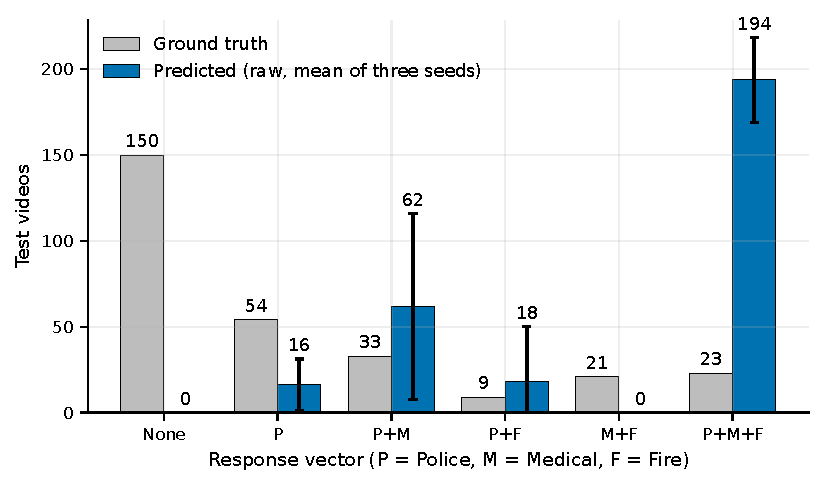
\includegraphics[width=0.88\textwidth]{fig_response_vector_distribution_r20.pdf}
    \caption[Predicted and ground-truth response vectors.]{Raw predicted response vectors (fixed bags, threshold 0.5, no gate; mean and sample SD over three seeds) beside the ground-truth vectors of the 290 test videos.}
    \label{fig:results-joint-dispatch}
\end{figure}

Aggregate metric stability did not imply stable per-video routing. Binary predictions were unanimous across seeds for 95.2\% of test videos, whereas the complete three-bit response vector was unanimous for 51.4\% (Table~\ref{tab:results-unanimity}). Channel-wise unanimity was 100.0\% for Police, 67.6\% for Medical, and 63.4\% for Fire.

\begin{table}[tbp]
    \centering
    \small
    \caption[Cross-seed unanimity of test predictions.]{Share of the 290 fixed-bag test videos on which all three seeds give the same prediction. The complete Police agreement follows from Police being predicted for every video, not from discriminative routing.}
    \label{tab:results-unanimity}
    \begin{tabular}{@{}lc@{}}
        \toprule
        \textbf{Output} & \textbf{Unanimous across seeds (\%)} \\
        \midrule
        Binary decision & 95.2 \\
        Complete response vector & 51.4 \\
        Police & 100.0 \\
        Medical & 67.6 \\
        Fire & 63.4 \\
        \bottomrule
    \end{tabular}
\end{table}

\section{Binary-Gated Routing and Matched Baselines}
\label{sec:results-fixed-routing}
\label{sec:results-fixed-baselines}

Restricting the same raw outputs to the 140 ground-truth anomalous videos increased Macro-F1 to $0.743 \pm 0.013$ (Table~\ref{tab:results-fixed-routing}). This is an oracle-conditioned diagnostic: normal videos and their false-positive opportunities are absent. Applying the learned binary gate over all 290 videos produced Macro-F1 $0.662 \pm 0.022$, reduced Hamming loss from $0.592 \pm 0.033$ to $0.234 \pm 0.016$, and increased exact match from $0.099 \pm 0.020$ to $0.545 \pm 0.009$ on the matched population.

The learned routing views were compared with all-services rules on the same populations. On all 290 videos, always predicting every service obtained Macro-F1 0.437, while the learned raw output obtained $0.478 \pm 0.009$. After using each checkpoint's binary decision, the learned response head obtained $0.662 \pm 0.022$, compared with $0.647 \pm 0.009$ for binary-gated all-services. On the 140 anomalous videos, learned raw routing obtained $0.743 \pm 0.013$, compared with 0.726 for the deterministic all-services rule. Table~\ref{tab:results-fixed-routing} also reports Hamming loss and exact match so that the comparison does not depend on Macro-F1 alone.

\begin{table}[tbp]
    \centering
    \footnotesize
    \caption[Matched fixed-bag routing conditions and baselines.]{Matched response-routing conditions on the test split using immutable 16-instance fixed bags. Learned channels and the learned raw part of the conditions use threshold 0.5; binary-gated rows use each checkpoint's binary argmax. The all-services rows are deterministic single rules and therefore carry no artificial SD, whereas learned and binary-dependent rows show mean $\pm$ sample SD across three checkpoints. The 140-video rows are ground-truth anomaly-conditioned diagnostics; all other rows use all 290 videos. No temporal cases are excluded.}
    \label{tab:results-fixed-routing}
    \begin{tabular}{@{}llccc@{}}
        \toprule
        \textbf{Population} & \textbf{Fixed-bag condition} & \textbf{Macro-F1} & \textbf{Hamming loss} & \textbf{Exact match} \\
        \midrule
        All 290 & Learned raw & $0.478 \pm 0.009$ & $0.592 \pm 0.033$ & $0.099 \pm 0.020$ \\
        All 290 & Learned binary-gated & $0.662 \pm 0.022$ & $0.234 \pm 0.016$ & $0.545 \pm 0.009$ \\
        All 290 & All services & 0.437 & 0.714 & 0.079 \\
        All 290 & Binary-gated all services & $0.647 \pm 0.009$ & $0.254 \pm 0.001$ & $0.534 \pm 0.000$ \\
        \addlinespace
        Anomalous 140 & Learned raw, oracle-conditioned & $0.743 \pm 0.013$ & $0.361 \pm 0.035$ & $0.205 \pm 0.041$ \\
        Anomalous 140 & All services & 0.726 & 0.407 & 0.164 \\
        Anomalous 140 & Binary-gated all services & $0.694 \pm 0.015$ & $0.418 \pm 0.013$ & $0.143 \pm 0.014$ \\
        \bottomrule
    \end{tabular}
\end{table}

The corresponding matched comparisons are small in Macro-F1: the fixed-bag learned gate exceeds binary-gated all-services by 0.015 (95\% video bootstrap interval 0.008 to 0.023), and anomaly-conditional learned routing exceeds all-services by 0.017. Per seed, the gated margin was 0.024, 0.000, and 0.022. For seed 2027, every video that passed the binary gate received all three services, so its gated output coincides with the binary-gated all-services rule on every test video, in the fixed-bag and the dense path alike. The mean margin therefore rests on two of the three checkpoints.

\section{Validation-Only Prototype-Distance Study}
\label{sec:results-ablation}

The $2\times2$ prototype-distance study comprises 12 validation runs: four variants, each trained with the same three seeds used by the official models. Table~\ref{tab:results-ablation} reports the fixed 161-video validation results. The highest mean response Macro-F1 was $0.452 \pm 0.008$ for No input, rather than the Full variant's $0.447 \pm 0.013$.

\begin{table}[tbp]
    \centering
    \small
    \caption[Validation-only prototype-distance study.]{Validation-only prototype-distance results on the immutable 161-video, 16-instance validation bags at response threshold 0.5; binary AUROC is threshold-free. Values are means and sample standard deviations across three training seeds. Checkpoints were selected and reported on this same validation population; none of the 12 runs loaded or evaluated the test split. The table therefore provides descriptive mechanism evidence, not test-performance or general causal evidence.}
    \label{tab:results-ablation}
    \begin{tabularx}{\textwidth}{@{}Xcccc@{}}
        \toprule
        \textbf{Variant} & \textbf{Macro-F1} & \textbf{Binary AUROC} & \textbf{Binary F1} & \textbf{Hamming loss} \\
        \midrule
        Full & $0.4474 \pm 0.0129$ & $0.9444 \pm 0.0002$ & $0.8590 \pm 0.0083$ & $0.5625 \pm 0.0371$ \\
        No input & $0.4520 \pm 0.0082$ & $0.9444 \pm 0.0007$ & $0.8518 \pm 0.0031$ & $0.5493 \pm 0.0303$ \\
        Uniform & $0.4393 \pm 0.0028$ & $0.9431 \pm 0.0002$ & $0.8502 \pm 0.0159$ & $0.5880 \pm 0.0198$ \\
        Neither & $0.4424 \pm 0.0077$ & $0.9415 \pm 0.0022$ & $0.8504 \pm 0.0138$ & $0.5769 \pm 0.0331$ \\
        \bottomrule
    \end{tabularx}
\end{table}

Guided sampling minus uniform sampling changed mean validation Macro-F1 by $+0.008$ when the score was appended and by $+0.010$ without score input. Appending the score changed the mean by $-0.005$ under guided sampling and by $-0.003$ under uniform sampling. With score input, the per-seed differences were $-0.0005$, $+0.019$, and $+0.006$, so guided sampling showed no consistent difference across seeds, and score concatenation did not improve the mean response Macro-F1 in this protocol. Selection on the reported validation set and the absence of test evaluation further preclude a causal conclusion.

\section{Normal-Bag Response-Loss Study (Validation Only)}
\label{sec:results-normal-bag}

The recorded validation history of the three official runs was checked first.
Police was predicted for all 161 validation videos at every logged epoch of
every run, and a minimum-Hamming-loss rule selects the official epoch in all
three runs. Intermediate checkpoints were not saved.

Table~\ref{tab:results-normal-bag} reports both loss variants against their
matched control on the 161-video validation set. \emph{Raw} is the ungated
response output on all videos; \emph{gated} applies each run's own binary
decision to both the learned output and the all-services reference;
\emph{anomalous-only} restricts to the 81 anomalous validation videos. Margins
are taken against the all-services reference of each view (raw 0.4046; gated
0.569--0.583, depending on the run's gate; anomalous-only 0.6520).

\begin{table}[tbp]
    \centering
    \small
    \caption[Normal-bag response-loss study, validation only.]{Normal-bag response-loss study, validation only. The first three columns are Macro-F1 margins over the matched all-services reference. Control is the Full arm of the prototype-distance study, without a normal-bag term; the unweighted variant adds normal bags to a single merged mean; the weighted variant adds them as a separate term ($\lambda=0.3$, fixed before training). Police and Medical precision/recall are on the raw output.}
    \label{tab:results-normal-bag}
    \begin{tabular}{@{}lccccc@{}}
        \toprule
        \textbf{Run} & \textbf{Raw} & \textbf{Gated} & \textbf{Anomalous} & \textbf{Police P / R} & \textbf{Medical P} \\
                     &              &                & \textbf{only}      & \textbf{(raw)}        & \textbf{(raw)} \\
        \midrule
        Control s1337    & +0.031 & +0.019 & +0.023 & 0.484 / 1.000 & 0.232 \\
        Control s2027    & +0.057 & +0.023 & +0.032 & 0.484 / 1.000 & 0.262 \\
        Control s3407    & +0.040 & +0.007 & +0.010 & 0.484 / 1.000 & 0.213 \\
        Unweighted s1337 & +0.184 & +0.007 & +0.015 & 0.735 / 0.962 & 0.390 \\
        Unweighted s2027 & +0.205 & +0.024 & +0.029 & 0.755 / 0.949 & 0.392 \\
        Unweighted s3407 & +0.189 & +0.017 & +0.025 & 0.735 / 0.962 & 0.380 \\
        Weighted s1337   & +0.164 & +0.019 & +0.032 & 0.685 / 0.974 & 0.356 \\
        Weighted s2027   & +0.177 & +0.020 & +0.032 & 0.681 / 0.987 & 0.372 \\
        Weighted s3407   & +0.169 & +0.017 & +0.034 & 0.658 / 0.987 & 0.372 \\
        \bottomrule
    \end{tabular}
\end{table}

Under the unweighted variant, raw Police precision rose from 0.484 (the
control, like the official checkpoints, predicted Police for all 161
validation videos) to 0.735--0.755, with recall falling from 1.000 to
0.949--0.962; false positives on the 80 normal validation videos fell from 80
to 21--24. Once both arms are gated identically, or restricted to the
anomalous videos, the variant's margin is indistinguishable within the
seed-to-seed spread from the control's (mean gated margin +0.016 in both
arms; mean anomalous-only margin +0.023 versus +0.022). Police still activates
on all three Explosion validation videos in every variant, the one category
the mapping assigns Police $=0$.

Against the unweighted variant, the weighted variant (Section~\ref{sec:normal-bag-study}) changed the margins as follows: the anomalous-only margin
rose by 0.0099, about 1.4 times the unweighted variant's seed standard
deviation of 0.0070, while the gated margin moved by 0.0026. Medical precision
fell by 0.021, Fire precision by 0.015, and Police precision by 0.067, about
six times the unweighted variant's spread; mean raw Macro-F1 was 0.574 versus
0.597. No other weight was tried.

\section{Dense Indexed-System and Temporal-Grounding Results}
\label{sec:results-dense-temporal}

\subsection{Dense Indexed Binary and Routing Results}

Table~\ref{tab:results-dense-routing} reports evaluation of the same three checkpoints on all 69,090 indexed test clips. Dense binary AUROC was $0.942 \pm 0.001$ and positive-class F1 was $0.874 \pm 0.010$. Raw, binary-gated, and anomaly-conditional response Macro-F1 values were $0.473 \pm 0.010$, $0.660 \pm 0.020$, and $0.740 \pm 0.012$, respectively. These values remain distinct from the fixed-bag results because every video's input bag changed.

\begin{table}[tbp]
    \centering
    \small
    \caption[Dense indexed binary and response results.]{Dense indexed-system results on the test split (variable-length bags, all 69,090 clips of the 290 videos). Binary AUROC is threshold-free; the other binary metrics use argmax; response metrics use threshold 0.5, with gating stated per block. The SD is the sample SD over the three Stage-2 seeds. The 140-video rows are oracle anomaly-conditioned and include the five videos with annotation-boundary conflicts.}
    \label{tab:results-dense-routing}
    \begin{tabular}{@{}lcccc@{}}
        \toprule
        \textbf{View and metric} & \textbf{Seed 1337} & \textbf{Seed 2027} & \textbf{Seed 3407} & \textbf{Mean $\pm$ sample SD} \\
        \midrule
        \multicolumn{5}{@{}l}{\emph{Binary, all 290 videos}} \\
        Accuracy & 0.883 & 0.872 & 0.886 & $0.880 \pm 0.007$ \\
        AUROC & 0.940 & 0.942 & 0.943 & $0.942 \pm 0.001$ \\
        Positive-class precision & 0.890 & 0.899 & 0.885 & $0.891 \pm 0.007$ \\
        Positive-class recall & 0.864 & 0.829 & 0.879 & $0.857 \pm 0.026$ \\
        Positive-class F1 & 0.877 & 0.862 & 0.882 & $0.874 \pm 0.010$ \\
        \addlinespace
        \multicolumn{5}{@{}l}{\emph{Response raw, all 290 videos}} \\
        Macro-F1 & 0.483 & 0.464 & 0.470 & $0.473 \pm 0.010$ \\
        Hamming loss & 0.571 & 0.639 & 0.609 & $0.607 \pm 0.034$ \\
        Exact match & 0.114 & 0.083 & 0.090 & $0.095 \pm 0.016$ \\
        \addlinespace
        \multicolumn{5}{@{}l}{\emph{Response binary-gated, all 290 videos}} \\
        Macro-F1 & 0.671 & 0.638 & 0.672 & $0.660 \pm 0.020$ \\
        Hamming loss & 0.225 & 0.253 & 0.230 & $0.236 \pm 0.015$ \\
        Exact match & 0.552 & 0.534 & 0.545 & $0.544 \pm 0.009$ \\
        \addlinespace
        \multicolumn{5}{@{}l}{\emph{Response raw, 140 anomalous videos}} \\
        Macro-F1 & 0.751 & 0.727 & 0.743 & $0.740 \pm 0.012$ \\
        Hamming loss & 0.340 & 0.402 & 0.362 & $0.368 \pm 0.031$ \\
        Exact match & 0.236 & 0.171 & 0.186 & $0.198 \pm 0.034$ \\
        \bottomrule
    \end{tabular}
\end{table}

The dense all-services baseline remained at Macro-F1 0.437. Dense binary-gated all-services reached $0.646 \pm 0.008$, compared with $0.660 \pm 0.020$ for learned binary-gated routing on all 290 videos. On the conditional 140-video population, all services reached 0.726, binary-gated all services reached $0.692 \pm 0.012$, and learned raw routing reached $0.740 \pm 0.012$. Figure~\ref{fig:results-routing-comparison} places these dense results beside their fixed-bag counterparts under matched populations.

\begin{figure}[tbp]
    \centering
    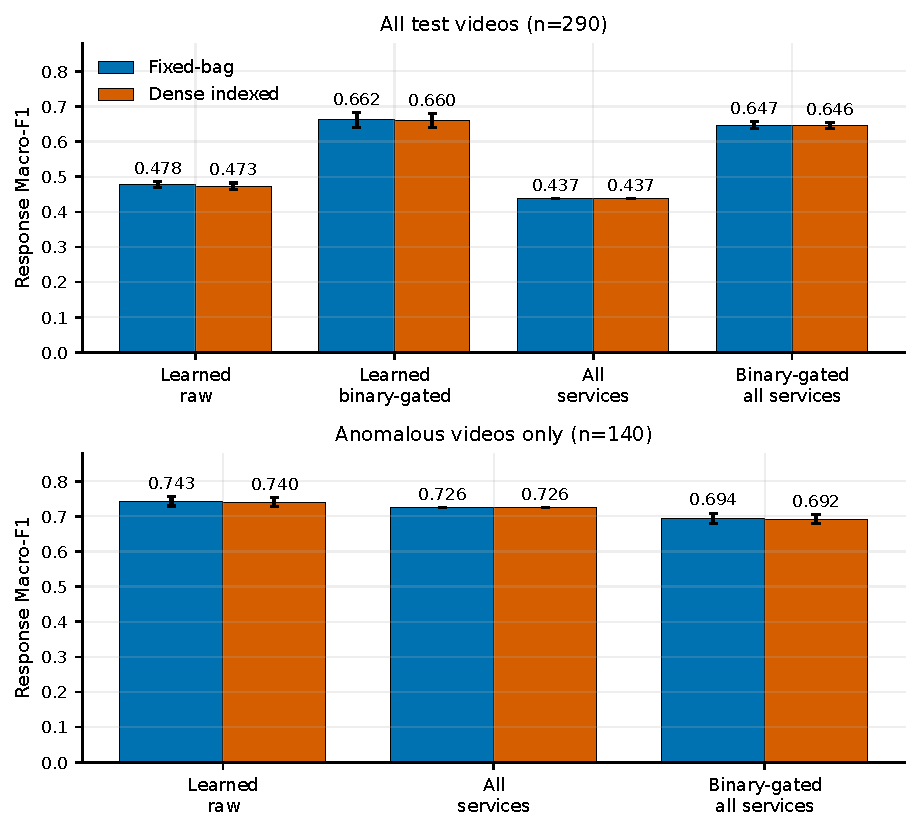
\includegraphics[width=\textwidth]{fig_routing_comparison_r20.pdf}
    \caption[Matched fixed-bag and dense routing comparisons.]{Response Macro-F1 of learned outputs and all-services rules on the fixed-bag and dense indexed inputs (threshold 0.5; gated conditions use the binary argmax). Top: all 290 test videos. Bottom: the 140 anomalous videos, an oracle-conditioned diagnostic. Error bars: sample SD over three seeds; all-services is one deterministic rule.}
    \label{fig:results-routing-comparison}
\end{figure}

\subsection{Dense Coverage}

The realized dense store covered 1,110,064 of 1,111,808 source frames, or 99.843\% frame-weighted coverage. Its mean per-video coverage was 99.540\%, the median was 99.758\%, and the minimum was 92.903\%. All annotated frames in the 135 temporally eligible anomaly videos were covered. Under the same source-frame geometry, sparse-store and fixed-bag frame-weighted coverage were 50.896\% and 12.062\%, respectively. These quantities describe which frames could be observed by each input construction; they are not performance metrics.

\subsection{Primary Temporal Grounding}

On the 135 source-bounded anomalous videos, mean temporal AP was $0.327 \pm 0.014$ and top-clip hit rate was $0.291 \pm 0.004$. At the primary interval threshold of 0.5, fixed before the dense evaluation, mean IoU was $0.186 \pm 0.017$ and $0.193 \pm 0.053$ of eligible videos had exactly zero IoU. The fractions with IoU of at least 0.1, 0.3, 0.5, and 0.7 were $0.558 \pm 0.026$, $0.215 \pm 0.032$, $0.074 \pm 0.007$, and $0.022 \pm 0.000$, respectively.

The separate binary-gated display rule at temporal threshold 0.65 produced mean IoU $0.128 \pm 0.014$ and zero-IoU frequency $0.425 \pm 0.045$. On the 150 normal videos, the ungated primary rule produced at least one interval for every video and assigned $0.379 \pm 0.056$ of source frames to predicted support. The binary-gated display rule produced at least one interval for $0.098 \pm 0.010$ of normal videos and assigned $0.026 \pm 0.006$ of their source frames to predicted support.

Temporal AP varied across the anomaly categories, whose test supports range from 2 to 23 videos; the per-category values are shown in Appendix Figure~\ref{fig:results-temporal-category}.

\subsection{Frozen Temporal References}

Table~\ref{tab:results-temporal-baselines} compares the learned attention with the four checkpoint-independent references. The whole-video reference scores every frame equally, so its AP equals the mean event prevalence of 0.191 and marks the chance level of AP. The learned model's temporal AP exceeded each reference; its mean gap to the whole-video reference was 0.136 (95\% video bootstrap interval 0.110 to 0.164). Its primary fixed-rule IoU was below the whole-video reference by 0.005 and above the random-clips and prototype-distance references. The uniform-clips rule had AP 0.192 but produced an empty interval after constant-score normalization for every eligible video, giving IoU zero and a zero-IoU frequency of one. The whole-video reference had zero zero-IoU cases because it always predicts the complete source duration.

\begin{table}[tbp]
    \centering
    \small
    \caption[Dense temporal model and frozen references.]{Temporal grounding on the 135 source-bounded anomalous test videos using the 69,090-clip dense indexed input; five boundary-conflict videos are excluded only here. AP and top-clip hit are threshold-free. Learned fixed-rule IoU uses the 0.5 temporal threshold and is summarized as mean $\pm$ sample SD across three checkpoints. Each reference is one frozen checkpoint-independent replicate under the same geometry and receives no fabricated SD; uniform constant scores yield empty predicted intervals by rule. No response threshold or binary gate is applied.}
    \label{tab:results-temporal-baselines}
    \begin{tabular}{@{}lcccc@{}}
        \toprule
        \textbf{Temporal method} & \textbf{AP} & \textbf{Top-clip} & \textbf{Fixed-rule} & \textbf{Zero-IoU} \\
                                  &              & \textbf{hit}      & \textbf{IoU}        & \textbf{frequency} \\
        \midrule
        Learned attention & $0.327 \pm 0.014$ & $0.291 \pm 0.004$ & $0.186 \pm 0.017$ & $0.193 \pm 0.053$ \\
        Whole video & 0.191 & --- & 0.191 & 0.000 \\
        Uniform clips & 0.192 & 0.015 & 0.000 & 1.000 \\
        Seeded random clips & 0.246 & 0.200 & 0.161 & 0.067 \\
        Prototype distance & 0.277 & 0.244 & 0.110 & 0.363 \\
        \bottomrule
    \end{tabular}
\end{table}

\section{Qualitative Success and Failure Cases}
\label{sec:results-qualitative}

Figure~\ref{fig:results-qualitative} shows four seed-1337 dense records chosen by fixed rules rather than by inspection. The \emph{best case} is the eligible anomalous video with the highest primary IoU among those with a correct binary decision and an exactly correct gated response vector. The \emph{median case} has the median primary IoU of the 135 eligible videos. The \emph{confident misplaced detection} is the zero-IoU video with the highest binary score, and the \emph{false alarm} is the normal video with the highest binary score. Ties are broken by video identity.

\begin{figure}[tbp]
    \centering
    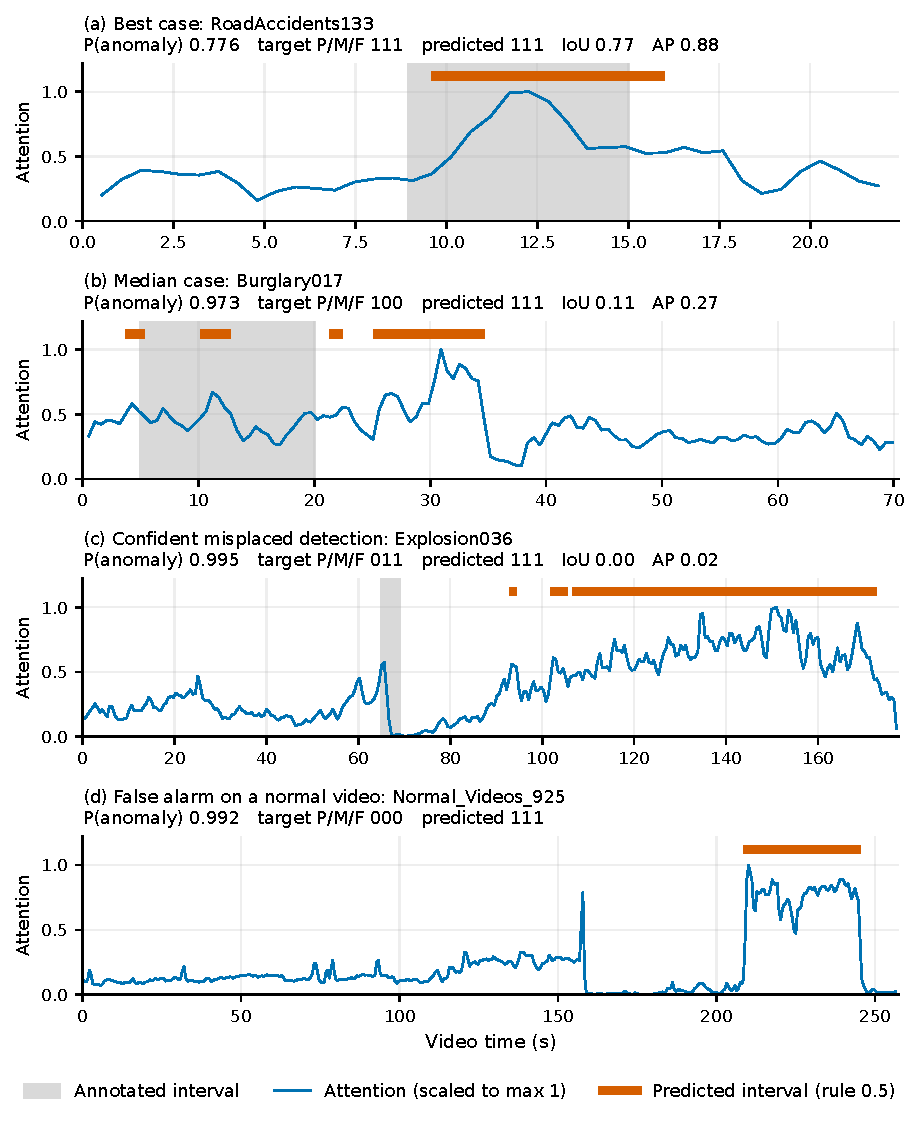
\includegraphics[width=\textwidth]{fig_qualitative_cases_r20.pdf}
    \caption[Qualitative success and failure cases.]{Four seed-1337 dense test records selected by the rules in Section~\ref{sec:results-qualitative}. Each panel shows the attention per clip (scaled to its maximum), the annotated interval, and the interval predicted by the primary rule. Target and predicted response vectors are given as Police/Medical/Fire bits. The videos are from UCF-Crime \cite{sultani2018real}.}
    \label{fig:results-qualitative}
\end{figure}

In the best case, \code{RoadAccidents133}, attention peaks at 12.3\,s inside the annotated interval of 9.0--15.0\,s, and the predicted interval of 9.6--16.0\,s gives IoU 0.77 and AP 0.88. Its correct response vector contains all three services, which is the vector the all-services rule would also produce. In the median case, \code{Burglary017}, the annotated interval is 5.0--20.0\,s, but attention peaks at 30.9\,s; the four predicted intervals overlap the event only in part, giving IoU 0.11, and the response vector adds Medical and Fire to the target Police. In \code{Explosion036}, the binary score is 0.995, but the annotated event lasts from 65.0 to 69.0\,s, while all predicted intervals lie between 92.8 and 172.8\,s; Police is predicted although the mapping assigns no Police to Explosion. The normal video \code{Normal\_Videos\_925} receives a binary score of 0.992, all three services, and a predicted interval of 208.5--245.3\,s.

\section{Offline CAD-Style Example}
\label{sec:results-cad-example}

Figure~\ref{fig:results-cad-example} presents the CAD-style record of a fixed example: the lexicographically first eligible anomalous seed-1337 output that triggered an alert, \code{Abuse/Abuse028\_x264.mp4}. Temporally, this example is a failure case. The dense bag contains 87 clips and covers 1,408 of 1,412 source frames. The target response is Police and Medical. The binary anomaly score is 0.897 and the binary decision is Anomaly. At the scientific response threshold of 0.5, the response vector is Police, Medical, and Fire. At the separate display thresholds $[0.65,0.60,0.65]$, the CAD-style record retains Police and Medical and assigns \code{P1-MEDICAL}.

The source-bounded annotation is frames $[164,240)$, while the primary 0.5 temporal rule predicts $[0,176)$ and $[320,352)$, giving IoU 0.044. The display rule predicts $[0,160)$ and therefore has IoU zero. Its displayed window is 0.00--5.33 seconds, whereas the annotated interval begins at 5.47 seconds: the alert is raised from the first second of the video, before the annotated event has begun. The stored \code{alert\_latency\_sec} is 0.00 because it records the displayed source-video timestamp, not computation time or delay from event onset.

\begin{figure}[tbp]
    \centering
    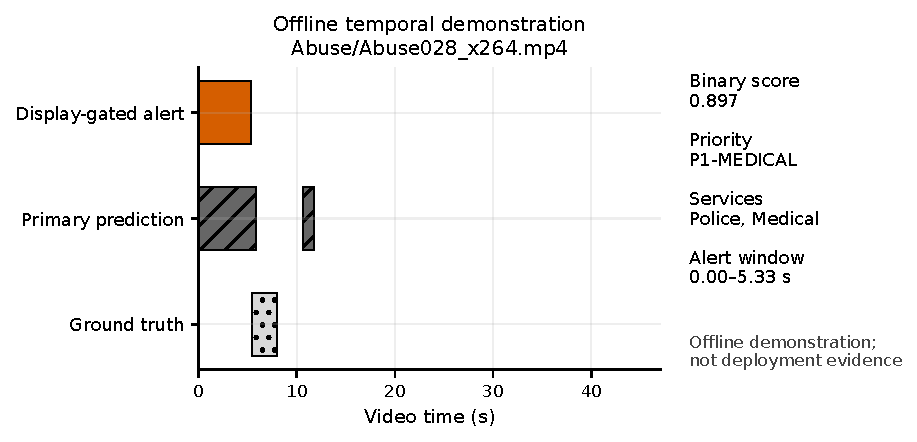
\includegraphics[width=\textwidth]{fig_temporal_cad_example_r20.pdf}
    \caption[Qualitative offline CAD-style record.]{Offline seed-1337 example for \code{Abuse/Abuse028\_x264.mp4}, selected by a deterministic lexical rule rather than performance; temporally a failure case (primary IoU 0.044). The dense input has 87 clips; the primary temporal rule uses threshold 0.5, while the displayed interval uses threshold 0.65 and the binary gate. Scientific response decisions use threshold 0.5; the displayed Police/Medical/Fire thresholds are $[0.65,0.60,0.65]$. This is one saved test record with no replicate uncertainty. It demonstrates deterministic rendering of model output, not live latency, external CAD integration, reliability, or safety.}
    \label{fig:results-cad-example}
\end{figure}

Figure~\ref{fig:results-cad-frame} shows the same record as an operator-facing overlay rendered on the source frame, rather than the schematic timeline above.

\begin{figure}[tbp]
    \centering
    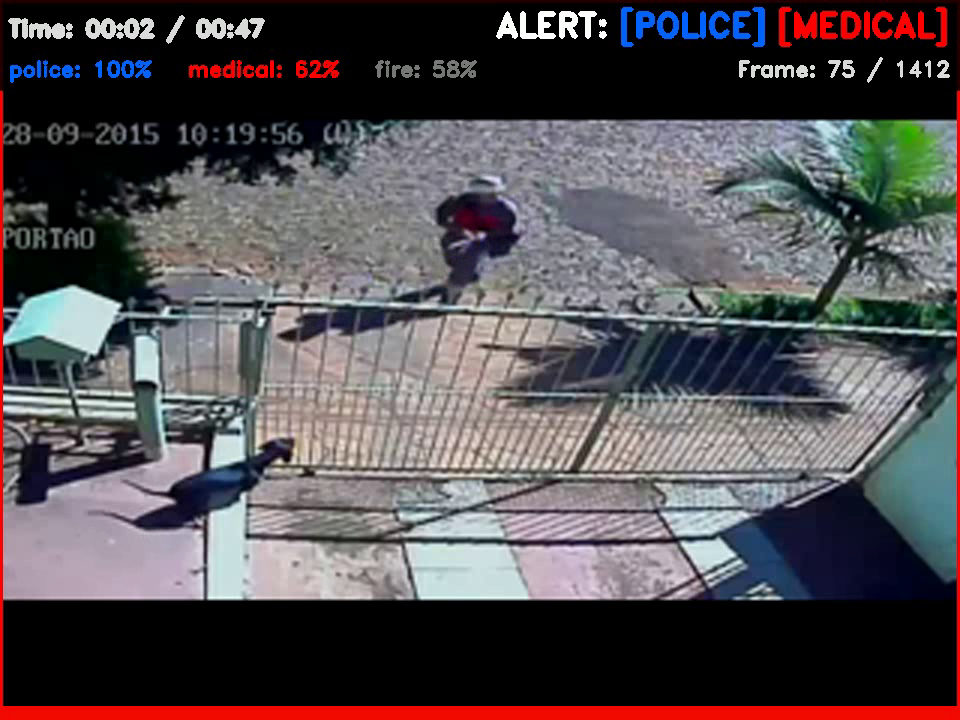
\includegraphics[width=0.8\textwidth]{fig_cad_frame_example.png}
    \caption[Rendered CAD-style overlay, source frame.]{Source-video frame at time 2.50\,s for the same \code{Abuse/Abuse028\_x264.mp4} seed-1337 example, inside the displayed alert window $[0.00,5.33]$\,s, rendered by the offline overlay tool (checkpoint \code{dispatch\_repro\_s1337}) rather than the fixed-bag or dense evaluation pipelines. Displayed confidences are rounded (police 100\%, medical 62\%, fire 58\%) from the same values as Figure~\ref{fig:results-cad-example}. This is UCF-Crime surveillance footage of a real scene \cite{sultani2018real}, shown once as a rendering example; it is not a live capture and is not deployment or safety evidence.}
    \label{fig:results-cad-frame}
\end{figure}

Figure~\ref{fig:results-cad-json} shows the stored alert record for the same example. It holds one alert window given by start and end frame, the dispatched services, the priority, and the per-channel confidences. It does not hold per-frame labels or an anomaly category.

\begin{figure}[tbp]
    \centering
    \begin{minipage}{0.75\textwidth}
\begin{lstlisting}[basicstyle=\ttfamily\footnotesize]
{
  "timestamp": "2026-09-27T10:13:59.510023",
  "source_video": "data/ucf_crime/raw/Abuse/
                   Abuse028_x264.mp4",
  "alert_triggered": true,
  "dispatch": ["police", "medical"],
  "priority": "P1-MEDICAL",
  "anomaly_window": {
    "start_frame": 0,
    "end_frame": 159,
    "start_sec": 0.0,
    "end_sec": 5.33
  },
  "confidence": {
    "police": 0.9994,
    "medical": 0.6235,
    "fire": 0.5785
  },
  "alert_latency_sec": 0.0
}
\end{lstlisting}
    \end{minipage}
    \caption[Stored alert record for the CAD-style example.]{Alert record stored for the same \code{Abuse/Abuse028\_x264.mp4} seed-1337 example (checkpoint \code{dispatch\_repro\_s1337}), with the \code{dispatch} list written on one line and the source path wrapped for width; all values are as stored. The window is stored as inclusive frames 0--159, which is the half-open interval $[0,160)$ used in the text. The record names the dispatched services, not an anomaly category.}
    \label{fig:results-cad-json}
\end{figure}

\section{Factual Summary}
\label{sec:results-summary}

Binary detection was consistent across the three checkpoints and both input paths, with an AUROC near 0.94 and a positive-class F1 near 0.87. The ungated response head had near-complete recall but low precision, and it predicted Police for every video. Binary gating improved all response metrics, yet the learned gated Macro-F1 stayed only slightly above the gated all-services rule. The two validation-only studies showed no consistent effect of guided sampling, of appending the distance, or of adding normal bags beyond removing the universal Police output. On the dense protocol, which covers 99.843\% of the test-video frames, temporal attention reached an AP of 0.327 and an IoU of 0.186, with 19.3\% of eligible videos at zero IoU. The four qualitative cases show one well-localized event and three confident decisions with misplaced intervals or a false alarm.
